\documentclass[fleqn,10pt]{wlscirep}
\usepackage[utf8]{inputenc}
\usepackage[T1]{fontenc}
\usepackage{ulem}
\newcommand{\li}{\uline{\hspace{0.5em}}}
\usepackage{amssymb}
\usepackage{amsmath}
\title{Analysis and Prediction of League of Legends Based on Machine Learning}

\author{ Fenghua Zhang, Weilin Tong}
\begin{abstract}
In this League of Legends World Tournament, KFC and the Tournament used deep learning to predict the strength of the hero lineup and the winning percentages of different periods. We envision whether such a winning rate prediction can be applied to the daily games of our average players. If we use match data from different regions in different regions, can we establish a real-time winning rate prediction for ordinary games? 

We used the crawler to collect the game data of the different leagues of the League of Legends statistics website, and then use the python implementation of xgboost to build our training test model, cross-validate and test our data. The Xgboost model achieves an accuracy of about 65\% on the test data. In view of the increased investigation accuracy as the number of samples increases, the model may perform better in the future as more game data increases.

\end{abstract}
\begin{document}

\flushbottom
\maketitle

\thispagestyle{empty}


\subsection*{Background}
League of Legends is a 3D, third person multiplayer online battle arena (MOBA) game. The game includes three currently running game modes: the Ripper's Rift, the Twisted Trunk, and the Howling Abyss. Players participate in the competition and last an average of 20 to 60 minutes. In each game mode, the team works together to achieve a winning condition, usually destroying the core building of the enemy team base (called Nexus) after bypassing a series of defensive structures called turrets or towers.

In all game modes, the player controls a character called a hero, selects or assigns each game, and each character has a unique set of abilities. The hero starts each game with a low level and then gains experience during the game to reach the highest level 18. Earning the hero level in the game allows the player to unlock their hero's special abilities and add them in a variety of unique ways. If a hero loses all his health, they will be defeated, but after enough time, they will automatically resurrect at their own base. Players can also start each game with a small amount of gold, and can get extra gold in the game in a variety of ways: by killing non-player characters called minions and monsters; killing or killing enemy by killing or helping Players; by destroying the structure of the enemy; passively over time; and gaining heroic abilities through unique project interactions. You can then spend all of the gold in the game to purchase items in the game, further increasing the abilities and games of each hero's various ways. The hero experience, the gold coins and the purchased items are unique to each game and will not be extended to subsequent games. Therefore, all players will start each game on an equal basis with respect to the opposing team.

In this project, we mainly study the competition mode of Summoner's Rift. Summoner's Rift is the most popular map in the League of Legends. In this map type, two teams of five players compete to destroy an enemy building called Nexus, which is guarded by enemy teams and some defensive structures called turrets or towers. A connection point is located at each enemy base on either side of the map, in the lower left corner and upper right corner. These structures continue to produce weak, non-player characters, called creeps, that follow three paths to the enemy base: the top, middle, and bottom channels. Players compete to push the waves of these creeps into the enemy base, which allows them to destroy the enemy's structure and eventually win the game.

\section*{Introduction and Related Work}

In this League of Legends World Tournament, KFC and the Tournament used deep learning to predict the strength of the hero lineup and the winning percentages of different periods. We envision whether such a winning rate prediction can be applied to the daily games of our average players. If we use match data from different regions in different regions, can we establish a real-time winning rate prediction for ordinary games? This is worth exploring, and it is a very valuable thing for our own players.

Project object: different levels of competition in different regions of the League of Legends;

Project problem solving:

\begin{itemize}
\item Real-time winning rate prediction for the game, providing an auxiliary reference to the audience;
\item After the game, give the player a prediction of the winning percentage in different periods of the game, and assist the post-match analysis to facilitate progress;
\end{itemize}



\section*{Data source and Pretreatment}

 At the beginning of the project, we used manual records to record the game data from the official and surrounding students of Lol, and found that there was a lot of invisible important information missing, which made our feature capture not comprehensive enough. At the same time, the manual crawling method is time-consuming and laborious, so discard and use the unofficial statistics that directly crawl the statistical website and make the feature data set belonging to us.

All data we use is available on the website Oracle's Elixir (https://oracleselixir.com/statistics/player-stats/). We use the matching data from 2016-2018 to carry out the project. This match data contains game statistics from players and teams from most leagues.

We found in the statistics that there are 83 characteristic information in the 2016 competition data, 99 in 2017 and 105 in 2018. As time goes on, more and more functions are collected. We will only use the same 64 feature information for all 3 years (the definition of the meaning of these features will be attached to the code):

\begin{figure}[ht]
\centering
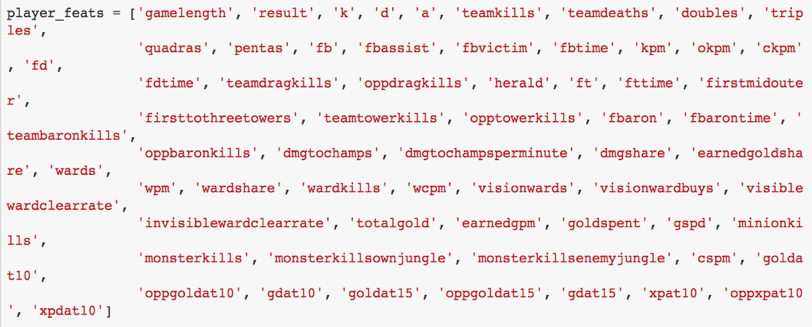
\includegraphics[width=\linewidth]{1.png}
\caption{64 features information}
\label{fig:1}
\end{figure}

For each game, we will generate features (weighted performance indicator for each player hero until the game) and use the blue side (ie the team starting at the bottom of the map) to win as a label (if the blue team wins, it is 1; if If the red team wins, it is 0). For each role in the team (Top, Jungle, Middle, ADC, and Support), we will generate weighted statistics for the players in that character. Therefore, for a game, we will provide 64 features for each player, and 10 players will have a total of 640 features. We built a crawler program for the above website to crawl a lot of game data on the website, and use sqlite3 to create a corresponding db file. (For specific crawlers and database programs see /utils/)

\subsection*{Proposed Method}

Before trying to use xgboost, I tried several different models (Logit, Random Forest, Adaboost). After comparing various algorithm models, we chose xgboost because of its speed and performance better than other algorithms. Below we list some of the advantages of xgboost:
\begin{itemize}
\item 1. Regularization
XGBoost adds a regular term to the cost function to control the complexity of the model. The regular term contains the number of leaf nodes of the tree and the sum of the squares of the L2 norms of the score output on each leaf node. From the perspective of Bias-variance tradeoff, the regular term reduces the variance of the model, making the learned model simpler and preventing overfitting, which is also a feature of xgboost over traditional GBDT.
\item 2. Parallel processing
We know that the most time-consuming step in the decision tree learning is to sort the values ​​of the features (because the best segmentation point is determined). XGBoost pre-stages the data before training and saves it as a block structure. This structure is used repeatedly in iterations, greatly reducing the amount of calculation. This block structure also makes parallelism possible. When performing node splitting, it is necessary to calculate the gain of each feature, and finally select the feature with the largest gain to split, then the gain calculation of each feature can be multithreaded.
\item 3. Flexibility
XGBoost supports user-defined target functions and evaluation functions, as long as the second order of the objective function can be guided.
\item 4. Pruning
XGBoost first builds all subtrees that can be built from top to bottom, and then prunes from bottom to top. This is not easy to fall into a local optimal solution compared to GBM.
\item 5. Built-in cross-validation
XGBoost allows cross-validation to be used in each round of boosting iterations. Therefore, the optimal number of boosting iterations can be easily obtained. GBM uses grid search and can only detect a limited number of values.
\end{itemize}

In short, xgboost is a collection method that uses a decision tree that iteratively adapts to weak learners using gradient enhancements to correct previous learner errors.


\section*{Model Construction}


We used Python's xgboost library for modeling. When tuning xgboost, we found that the parameters of xgboost are more complicated, and it is difficult to find a good tuning rule in a short time. Therefore, after deliberation, we decided to use the enumeration method to adjust the parameters. We first made a certain attempt around the default parameters of xgboost, determined the reasonable range of each parameter, and then selected 3~4 candidate values in this range, and used the loop to obtain the optimal parameters for these candidate values. The parameters and their candidate values are set as follows (Table 1):

\begin{table}[ht]
\centering
\begin{tabular}{|p{5cm}|p{5cm}|p{5cm}|}
\hline
Parameter & Candidate value & Meaning \\
\hline
max\li depth (default=6) & 1,2,3 & The maximum depth of the tree, the larger the max\li depth, the model will learn more specific and more local samples, and it will be easier to overfit. \\
\hline
learning\li rate (default=0.3) & 0.1, 0.05, 0.01 & Learning rate\\
\hline
n\li estimators
[default=100]&
80, 100, 120&
Increase the number of trees\\
\hline
gamma(default=0)&
0.0, 0.1, 0.03, 0.01&
When the node splits, the node will split the node only if the value of the post-split loss function drops. The gamma formulates the minimum loss function drop value required for node splitting. The larger the value, the more conservative the algorithm\\
\hline
min\li child\li weight
(default=1)&
0, 1, 2, 3&
Determine the minimum leaf node sample weight sum, when its value is large, you can avoid the model learning local special samples, and it is easier to avoid over-fitting\\
\hline
max\li delta\li step
(default=0)&
0, 1, 2, 3&
This parameter limits the maximum step size for each tree weight change. If this parameter is 0, it means there is no limit. If it is a positive value, it will make the algorithm more conservative\\
\hline
Subsample
(default=1)&
1.0, 0.9, 0.5&
Control the proportion of random samples for each tree. Decreasing this parameter will make the algorithm more conservative and avoid over-fitting, but if it is too small, it will lead to under-fitting\\
\hline
reg\li alpha
(default=0)&
0.0, 0.01, 0.03, 0.01&
The L1 regularization of the weights. The larger the value, the more conservative the algorithm\\
\hline
reg\li lambda
(default=1)&
1.0, 0.5, 0.9&
The L2 regularization of the weights. The larger the value, the more conservative the algorithm\\
\hline
\end{tabular}
\caption{\label{tab:example}Parameters setting.}
\end{table}
	We spent about 2 days for enumeration, and finally found the parameters as ["max\li depth":1, "n\li estimators":100, "learning\li rate":.1, "colsample\li bytree": .5, "subsample": . 5, "gamma": 0] a set of parameters perform best.
	
The sample performance is:
\begin{figure}[ht]
\centering
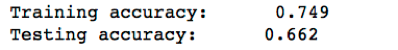
\includegraphics[width=\linewidth]{2.png}
\caption{Test performance }
\label{fig:2}
\end{figure}

Then we found two parameter-optimized available functions in the sklearn.model\li selection library (grid search GridSearchCV, random search RandomizedSearchCV) and conducted related tests (figure 3):
\begin{figure}[ht]
\centering
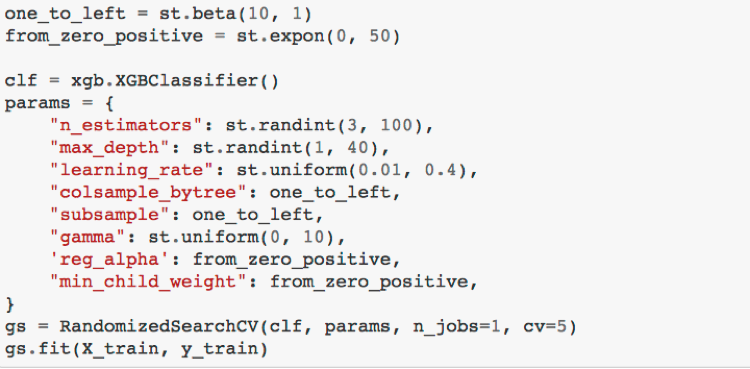
\includegraphics[width=\linewidth]{3.png}
\caption{RandomizedSearchCV}
\label{fig:3}
\end{figure}

Here we use the random search RandomizedSearchCV for tuning:

RandomizedSearchCV implements a random search of parameters, each of which is sampled from a distribution of possible parameter values. This has two main advantages for exhaustive search:
\begin{itemize}
\item 1. You can choose a budget that is independent of the number of parameters and possible values;
\item 2. Adding parameters that do not affect performance does not reduce efficiency.

After a certain test we found the best combination of parameters for the model training:
['base\li score': 0.5, 'booster': 'gbtree', 'colsample\li bylevel': 1, 'colsample\li bytree': 0.95189402067426998, 'gamma': 3.4046372184882645, 'learning\li rate': 0.23949358694003495, 'max\li delta\li step': 0, 'max\li depth': 13 , 'min\li child\li weight': 4.6529230741397205, 'missing': None, 'n\li estimators': 27, 'nthread': 1, 'objective': 'binary:logistic', 'reg\li pos\li weight' : 1, 'seed': 0, 'silent': 1, 'subsample': 0.68356946419822784]

\end{itemize}



\section*{Experiments}

To evaluate the performance of our model, we first divided the matching data into training (70\%) and testing (30\%). The natural accuracy (maximum division) is about 55\%(that is, 55\% of all competitions are won by the Blue team) - this is due to the nature of the game, the so-called "blue side advantage" (blue team won the championship for the first time, so They often get the combination of heroes they want, and the red team has only a chance to fight back)

We used xgboost to cross-check the training set five times. The model achieved an average accuracy of approximately 63\% during cross-validation with a standard deviation of ~1.3\%. After that, I trained the model on the entire training set and assessed the accuracy of the training and test sets. The model achieved approximately 78\% accuracy on the training set and approximately 65\% accuracy on the test set. Therefore, the model is about 10\% better than natural.

At the same time, we use different data sets to carry out the training and verification of the model, and explore whether the accuracy has a great relationship with the size of the data set. The results of the investigation are as shown in the figure 4:
\begin{figure}[ht]
\centering
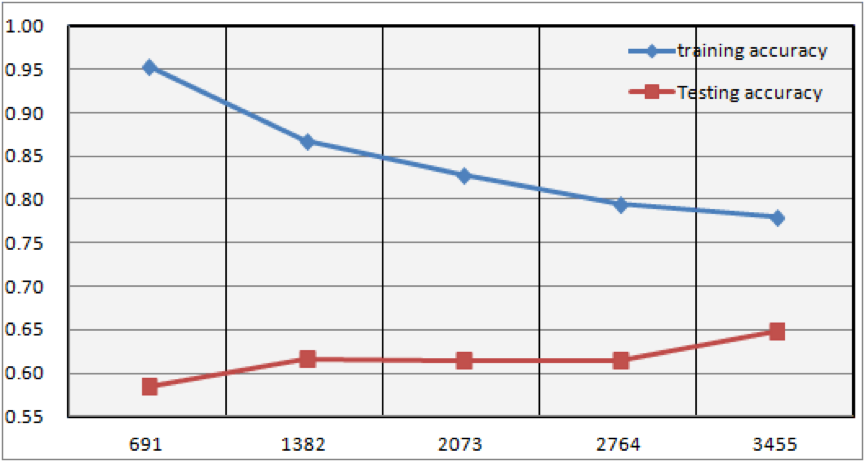
\includegraphics[width=\linewidth]{4.png}
\caption{The results of the investigation}
\label{fig:4}
\end{figure}

The results indicate and our conjecture: with a larger sample set, the accuracy of the model tends to increase, although the increase is not very large. This may mean that if we have more game data than we do now, the model might do better. It can be seen from the difference between training and test accuracy that the model is also slightly over-fitting. Further adjustments can be made later.


\section*{Result Analysis}

We will build a good xgboost model and use Logit, Random Forest to compare the horizontal model, and find that xgboost is the best in the data sample set.(figure 5)
\begin{figure}[ht]
\centering
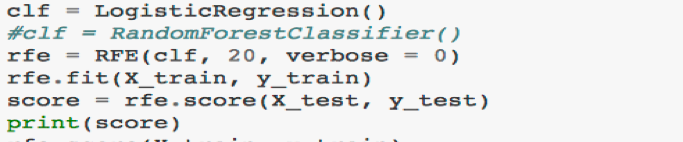
\includegraphics[width=\linewidth]{5.png}
\caption{Compare}
\label{fig:5}
\end{figure}

\begin{table}[ht]
\centering
\begin{tabular}{|p{5cm}|p{5cm}|}
\hline
Model & Score\\
\hline
Logistic Regression&
0.5639\\
\hline
Random Forest&
0.5811\\
\hline
Xgboost&
0.6482\\
\hline
\end{tabular}
\caption{\label{tab:example}Model Comparing.}
\end{table}

In addition, we examined the top 10 predictive features in the model (order of importance). Since the final model is a collection of trees, we can choose the functionality for creating the most informative segmentation. Fortunately, the xgboost library can do this automatically, the result is as follows(Tabel 3):

\begin{table}[ht]
\centering
\begin{tabular}{|p{5cm}|p{5cm}|}
\hline
Feature & Importance\\
\hline
blue\li Support\li gspd&
0.020528\\
\hline
red\li Middle\li gdat15 &
0.017595\\
\hline
blue\li ADC\li gspd&
0.017595\\
\hline
red\li Jungle\li fbaron&
0.011730\\
\hline
blue\li Support\li monsterkillsenemyjungle&
0.011730\\
\hline
red\li Top\li gspd&
0.011730\\
\hline
blue\li Support\li dmgtochamps&
0.011730\\
\hline
blue\li Middle\li gspd&
0.011730\\
\hline
red\li ADC\li result&
0.008798\\
\hline
blue\li Support\li xpdat10&
0.008798\\

\hline
\end{tabular}
\caption{\label{tab:example}Parameter Importance}
\end{table}

We have done some analysis of this result ourselves:
\begin{itemize}
\item 1. Analyzing the top ten predictive features, it seems that the performance of the blue-side down role (ADC and Support) seems to be the most important predictor of the outcome of the game. The ADC is usually the main damage in the team, and Support usually protects the ADC from safely attacking the attack and continually attacking in team battles. There is no doubt that players in these two roles are very important in predicting the outcome of the game. This result is in full compliance with the common sense of our regular competition.
\item 2. But to our surprise, Support is shown in this list very frequently (4/10). In general, Support usually helps their other team members, especially ADCs, who usually don't get a lot of coins or kills. But the predictions here clearly remind us that in a game, the role of Support is not particularly obvious, but the impact on the outcome of the entire game is very critical.
\item 3. In addition, “gspd” (the percentage difference in gold consumption, which is the percentage difference between gold spent between teams) has also appeared four times, which indicates that it is also crucial. GSPD usually measures the economic proximity of the two sides of the game: if the GSPD between the two teams is very low at the end of the game, then this means that they have little economic gap at the end of the game, meaning that the hero's equipment ability is not much different. . But if GSPD is high, then a team dominates the game, gaining and spending more money during the game, natural heroes have more equipment and abilities, the team gains more advantage and the winning percentage is higher.\\
\end{itemize}

\section*{Project Summary}

In summary, we used the crawler to collect the game data of the different leagues of the League of Legends statistics website, and then use the python implementation of xgboost to build our training test model, cross-validate and test our data. The Xgboost model achieves an accuracy of about 65\% on the test data. In view of the increased investigation accuracy as the number of samples increases, the model may perform better in the future as more game data increases.

Looking ahead, we may try to explore how different locations in the game work together better, and we need to study the heroes of different heroes for the entire game. In addition, we can continue to supplement the sample data and try to provide better win rate predictions using better neural networks (such as LSTM).

\end{document}